%!TEX TS-program = xelatex
\documentclass[]{friggeri-cv}
\usepackage{afterpage}
\usepackage{hyperref}
\usepackage{color}
\usepackage{xcolor}
\usepackage{smartdiagram}
\usepackage{fontspec}
% if you want to add fontawesome package
% you need to compile the tex file with LuaLaTeX
% References:
%   http://texdoc.net/texmf-dist/doc/latex/fontawesome/fontawesome.pdf
%   https://www.ctan.org/tex-archive/fonts/fontawesome?lang=en
%\usepackage{fontawesome}
\usepackage{metalogo}
\usepackage{dtklogos}
\usepackage[utf8]{inputenc}
\usepackage{tikz}
\usetikzlibrary{mindmap,shadows}

\usepackage{fontawesome}
\pdfmapfile{fontawesome.map}
\usepackage{makecell}

\newcommand{\WorkExpProject}[5]{
        & \makecell[r]{\em #1 \\ \bfseries #2}  & \bfseries #3 \\* 
        &Responsibilities & \small #4 \\*
        &Environment & \small #5 \\*
        \multicolumn{1}{c}{} \\
}

\hypersetup{
    pdftitle={},
    pdfauthor={},
    pdfsubject={},
    pdfkeywords={},
    colorlinks=false,           % no lik border color
    allbordercolors=white       % white border color for all
}
\smartdiagramset{
    bubble center node font = \footnotesize,
    bubble node font = \footnotesize,
    % specifies the minimum size of the bubble center node
    bubble center node size = 0.5cm,
    %  specifies the minimum size of the bubbles
    bubble node size = 0.5cm,
    % specifies which is the distance among the bubble center node and the other bubbles
    distance center/other bubbles = 0.3cm,
    % sets the distance from the text to the border of the bubble center node
    distance text center bubble = 0.5cm,
    % set center bubble color
    bubble center node color = pblue,
    % define the list of colors usable in the diagram
    set color list = {lightgray, materialcyan, orange, green, materialorange, materialteal, materialamber, materialindigo, materialgreen, materiallime},
    % sets the opacity at which the bubbles are shown
    bubble fill opacity = 0.6,
    % sets the opacity at which the bubble text is shown
    bubble text opacity = 0.5,
}

\addbibresource{bibliography.bib}
\RequirePackage{xcolor}
\definecolor{pblue}{HTML}{0395DE}

\begin{document}
\header{Artsiom}{Kaltovich}
      {Software Engineer}
      {Saint-Petersburg/Minsk}

% Fake text to add separator
\fcolorbox{white}{gray}{\parbox{\dimexpr\textwidth-2\fboxsep-2\fboxrule}{%
.....
}}

% In the aside, each new line forces a line break
\begin{aside}
  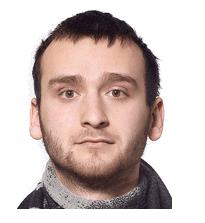
\includegraphics[width=4cm]{img/Artsiom_Kaltovich.jpg}
    ~
  \section{Qualifications}
      \smartdiagram[bubble diagram]{
          \textbf{Program}\\\textbf{ming},
          \textbf{Bioinformatics},
          \textbf{ML}\\\textbf{Statistic},
          \textbf{Data}\\\textbf{Structures},
          \textbf{Algorithms},
          \textbf{Python}
      }
    ~
  \section{Personal Skills}
    \smartdiagram[bubble diagram]{
        \textbf{Team}\\\textbf{Player},
        \textbf{Problem}\\\textbf{solver},
        \textbf{Respon}\\\textbf{sible},
        \textbf{Innova}\\\textbf{tive},
        \textbf{Ambitious},
        \textbf{Friendly}
    }
    ~
    \section{Languages}
        \textbf{Belarussian}
\includegraphics[scale=0.40]{img/5stars.png}
        \textbf{Russian}
\includegraphics[scale=0.40]{img/5stars.png}
        \textbf{English}
\includegraphics[scale=0.40]{img/4stars.png}
        \textbf{German}
\includegraphics[scale=0.40]{img/2stars.png}
    ~
    \section{Contacts}
     \small items are clickable, but not in github preview :)
    \begin{tabular}[\textwidth]{lp{4cm}}
        \large\textnormal{\faGithub} & {\href{https://github.com/\github}{\github}} \\[-0.4cm]
        \large\textnormal{\textcolor{kaggle}{\textbf{k}}} & {\href{https://www.kaggle.com/linearleopard}{linearleopard}}\\[-0.4cm]
        \large\textnormal{\textcolor{linkedin}{\faLinkedin}} & \href{https://www.linkedin.com/in/\linkedin}{\linkedin}\\[-0.4cm]
        \large\textnormal{\textcolor{gmail}{\faAt}} & \href{mailto:\mail}{\mail}\\[-0.4cm]
        %\large\textnormal{\textcolor{skype}{\faSkype}} & \href{skype:\skype?userinfo}{\skype}\\[-0.4cm]
    \end{tabular}
\end{aside}
~
\section{Experience}
\begin{tabular}{lrp{10cm}}
    \WorkExpProject{Sep 2019 - Dec 2020}
        {\makecell[r]{Software Engineer}}
        {Big Data Solutions}
        {Creating Pandas-like wrapper for OneTick database query language}
        {Python, OneTick, Sphinx, pytest, fintech}
    \WorkExpProject{Jun 2018 – Aug 2019}
        {\makecell[r]{Software Engineer}}
        {SK Hynix Memory Solutions Eastern Europe}
        {NAND Testing and Emulating. Creating model and software for emulating and testing NAND Firmware}
        {Python, C, C++, Perforce}
    \WorkExpProject{Dec 2017 – Jun 2018}
        {\makecell[r]{Software Engineer}}
        {Workfusion}
        {Training partners' students: creating samples, Q\&A sessions, course creating, grading assignments, troubleshooting.}
        {Java, Selemium, XML, Web-Harvest, WorkFusion}
    \WorkExpProject{Feb 2017 – Mar 2017}
        {\makecell[r]{Data Sciencer\\Python Developer}}
        {Remote work/side project}
        {Migrating pipeline of analyzing scientific data in bioinformatics research from R to Python. Visualizing data, p-value, correlation and other metrics calculation}
        {Linux, Python, R, Matplotlib, Biopython, Bokeh, PyPlot, sklearn, pandas}
    \WorkExpProject{Jun 2013 – Dec 2017}
        {Software Engineer}
        {IBA Group}
        {Support and maintenance of UDS/SQL. Developing extension for Eclipse IDE. Upgrading ERP-system from IBM Maximo 5 to Maximo 7.}
        {BS2000, COBOL, Assembler, SPL, Eclipse SDK and RCP, Java, SWT, JFace, Linux, WebSphere, JSP, XML, SQL, PHP, Perl}
\end{tabular}
\vspace{-0.5cm}
\section{Education}
    \begin{tabular}[\textwidth]{rp{10cm}}
        % Bionformatics Institute
        \em \makecell[r]{Sep 2019 - Dec 2020} & \textbf{Bionformatics Institute}, \textit{Saint-Petersburg} \\
        & Algorithmic Bioinformatics\\
        \multicolumn{1}{c}{} \\

        % bsuir
        \em \makecell[r]{Sep 2010 - Jun 2015} & \textbf{Belarusian State University of Informatics}\\\textbf{and Radioelectronics}, \textit{Minsk} \\
        Faculty & Computer System and Networks\\
        Department & Software for Information Technologies\\
    \end{tabular}\\
    
\section{Interests and Activities}

Programming, Mathematics, Physics, History, Languages, Economy, Politics.\\
Dancing, Cooking, Traveling.
\end{document}
